\section{450 --- Delete Node in a BST}
Given a root node reference of a BST and a key $x$, delete the node with the given key in the BST. Return the root node reference (possibly updated) of the BST.

Basically, the deletion can be divided into two stages:

\begin{itemize}
\item Search for a node to remove.
\item If the node is found, delete the node.
\end{itemize}

\paragraph{Note:} 
\begin{itemize}
\item Time complexity should be O(height of tree).
\end{itemize}

\paragraph{Example:}
\begin{flushleft}
\textbf{Input}: 
\begin{figure}[H]
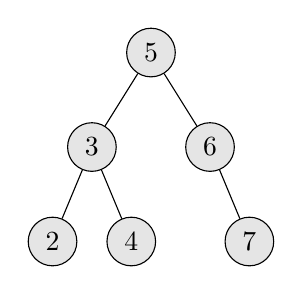
\begin{tikzpicture}
[every node/.style={draw, circle, fill=gray!20!, minimum size=5mm},
level 2/.style ={sibling distance=1cm}, 
level 3/.style={sibling distance=8mm},
level distance=1.2cm]
\node {5}
 child{ node(a){3} child { node {2} } child { node {4} }   } 
%
 child{ node(b){6} child[missing] {} child { node {7} } };
%;
\end{tikzpicture}
\end{figure}
$x = 3$

\textbf{Output}: 
One valid answer is shown in the following BST.

\begin{figure}[H]
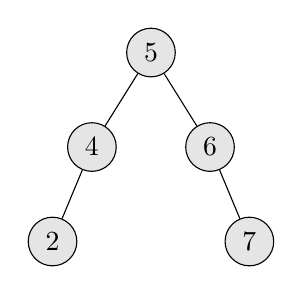
\begin{tikzpicture}
[every node/.style={draw, circle, fill=gray!20!, minimum size=5mm},
level 2/.style ={sibling distance=1cm}, 
level 3/.style={sibling distance=8mm},
level distance=1.2cm]
\node {5}
child { node {4} child {node{2}} child[missing]{} }
child { node {6} child[missing] {} child {node{7}} };
\end{tikzpicture}
\end{figure}

Another valid answer is
\begin{figure}[H]
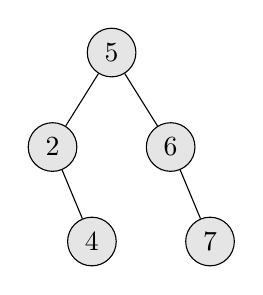
\begin{tikzpicture}
[every node/.style={draw, circle, fill=gray!20!, minimum size=5mm},
level 2/.style ={sibling distance=1cm}, 
level 3/.style={sibling distance=8mm},
level distance=1.2cm]
\node {5}
child { node {2} child[missing]{} child {node{4}} }
child { node {6} child[missing] {} child {node{7}} };
\end{tikzpicture}
\end{figure}
\end{flushleft}